\documentclass[12pt,letterpaper]{article}

\documentclass[12pt,letterpaper]{article}

\newenvironment{proof}{\noindent{\bf Proof:}}{\qed\bigskip}

\newtheorem{theorem}{Theorem}
\newtheorem{corollary}{Corollary}
\newtheorem{lemma}{Lemma} 
\newtheorem{claim}{Claim}
\newtheorem{fact}{Fact}
\newtheorem{definition}{Definition}
\newtheorem{assumption}{Assumption}
\newtheorem{observation}{Observation}
\newtheorem{example}{Example}
\newcommand{\qed}{\rule{7pt}{7pt}}

\newcommand{\homework}[4]{
	\thispagestyle{plain} 
	\newpage
	\setcounter{page}{1}
	\noindent
	\begin{center}
		\framebox{ \vbox{ \hbox to 6.28in
				{\bf CS 260: Machine Learning Algorithms\hfill #1} %change course name
				\vspace{4mm}
				\hbox to 6.28in
				{\hspace{2.5in}\large\mbox{Homework 2}}
				\vspace{4mm}
				\hbox to 6.28in
				{{\it Student Name: Abdullah-Al-Zubaer Imran#3\hfill UID: 804733867 #4}}
			}}
		\end{center}
	}
	
\newcommand{\quiz}[4]{
	\thispagestyle{plain} 
	\newpage
	\setcounter{page}{1}
	\noindent
	\begin{center}
		\framebox{ \vbox{ \hbox to 6.28in
				{\bf CS 260: Machine Learning \hfill #4}
				\vspace{4mm}
				\hbox to 6.28in
				{\hspace{2.5in}\large\mbox{Quiz \hfill #2    }}
				\vspace{4mm}
				\hbox to 6.28in
				{{\it Time: #3 \hfill Name:  #4 \hfill }}
			}}
		\end{center}
	}

\newcommand{\assignment}[4]{
	\thispagestyle{plain} 
	\newpage
	\setcounter{page}{1}
	\noindent
	\begin{center}
		\framebox{ \vbox{ \hbox to 6.28in
				{\bf CS 260: Machine Learning \hfill #1}
				\vspace{4mm}
				\hbox to 6.28in
				{\hspace{2.5in}\large\mbox{Homework #2}}
				\vspace{4mm}
				\hbox to 6.28in
				{{\it Handed Out: #3 \hfill Due: #4}}
		}}
	\end{center}
}

\newcommand{\exam}[4]{
	\thispagestyle{plain} 
	\newpage
	\setcounter{page}{1}
	\noindent
	\begin{center}
		\framebox{ \vbox{ \hbox to 6.28in
				{\bf CS 260: Machine Learning \hfill #4}
				\vspace{4mm}
				\hbox to 6.28in
				{\hspace{2.5in}\large\mbox{#2 \hfill  Exam }}
				\vspace{4mm}
				\hbox to 6.28in
				{{\it Time: #3 \hfill Name:  #4 \hfill }}
		}}
	\end{center}
}

\newenvironment{algorithm}
{\begin{center}
\begin{tabular}{|l|}
\hline
\begin{minipage}{1in}
\begin{tabbing}
\quad\=\qquad\=\qquad\=\qquad\=\qquad\=\qquad\=\qquad\=\kill}
{\end{tabbing}
\end{minipage} \\
\hline
\end{tabular}
\end{center}}

\def\Comment#1{\textsf{\textsl{$\langle\!\langle$#1\/$\rangle\!\rangle$}}}

%for different course, change the commented lines in this file
\usepackage{graphicx,amssymb,amsmath,bm}
\usepackage{newcommand}
\usepackage{mathtools}
\usepackage{amsmath}
\usepackage{dsfont}
\DeclarePairedDelimiter\ceil{\lceil}{\rceil}
\newcommand{\floor}[1]{\left\lfloor #1 \right\rfloor}

\sloppy
\newcommand{\ignore}[1]{}
\usepackage{hyperref}

\oddsidemargin 0in
\evensidemargin 0in
\textwidth 6.5in
\topmargin -0.5in
\textheight 9.0in

\begin{document}

\homework{Fall 2018}{$4$}{}{}
\begin{footnotesize}
	\begin{itemize}
		\item Feel free to talk to other students in the class when doing the homework. You should, however, write down your solution yourself. You also must indicate on each homework with whom you collaborated and cite any other sources you use including
		Internet sites.
		\item You will write your solution in LaTeX and submit the pdf file through Gradescope. You also need to submit the zipped LaTeX files to CCLE.
		We will grade your homework based on the final  version of the pdf file submitted to Gradescope. We will not grade the zipped Latex files on CCLE. However, failure to submitting your LaTax files to CCLE will incur 2 points penalty out of 100 points.	
				\item The homework (both pdf and zipped Latex source files) is due at 3:59 PM before the class.
	\end{itemize}
\end{footnotesize}


\begin{enumerate}
	

\item[1.] (10.1) \\
{\noindent}\textbf{Boosting the Confidence}\\
{\noindent}We divided the data into $k+1$ chunks i.e., $k=\ceil{\frac{\log(\delta/2)}{\log(\delta_0)}}$, with each chunk having the sample complexity $m_\mathcal{H}(\delta)$. Then applying the algorithm A to each of the chunks, we have
\begin{align*}
    &\mathbb{P}[\forall_i \in [k], L_{\mathcal{    D}}(A(\mathcal{S}_i)) > \min_{h\in\mathcal{H}}L_{\mathcal{D}}(h) + \epsilon]\\
    &=\prod_i \mathbb{P}[L_\mathcal{D}(A(\mathcal{S}_i)) > \min_{h\in\mathcal{H}}(h) + \epsilon]\\
    &< \delta_0^k\\
    &\leq \delta/2
\end{align*}

{\noindent}Using the algorithm A for the k+1 chunks and following the corollary 4.6, the best one is picked. This necessarily means denotes agnostic PAC learnability. So, for the agnostic PAC learnable class on $m\leq \ceil{\frac{2\log(4k/\delta)}{\epsilon^2}}$ samples, with probability of at least $1 - \delta/2$, we get

$$\mathcal{L}_\mathcal{D}(A(\mathcal{S}_i)) \leq \min_{h\in\mathcal{H}}\mathcal{L}_\maathcal{D}(h) + \epsilon$$ 

Hence with the union bound we can state that using the algorithm A, the hypothesis class $\mathcal{H}$ is agnostic PAC learnable with the sample complexity
\begin{align*}
    m_\mathcal{H}\epsilon, \delta) \leq km_\mathcal{H}(\delta) + \ceil{\frac{2\log(4k/\delta)}{\epsilon^2}}
\end{align*}



\clearpage

\item[2.] (12.1) \\
{\noindent}The 0--1 loss function is discrete. So, if there is an error for a data example, the loss can fluctuate jumping from 0 to 1 or vice-versa. This propoerty can break the convex function definition which makes 0--1 loss function no-convex. 

If we consider the homogeneous halfspace hypothesis class $\mathcal{H} = \{sign\langle \mathbf{w}, x\rangle\}$ with one training example. Whenever the hypothesis does not correctly classify this single training example, it will have a training loss $\mathcal{L}_S(\mathbf{w}) = 1$. Now, in the small vicinity, $\forall_\mathbf{w}', \|\mathbf{w}-\mathbf{w}'\| \leq \epsilon$. So, untill the decision boundary of the halfspace classifies this training example correctly, $\mathcal{L}_S(\mathbf{w}') = 1$. This means  $\mathbf{w}$ is actually a local minimum of $\mathcal{L}_S$. 

However, there exists some \mathbf{w}* (for example, increase or decrease $\mathbf{w}$ to correctly classify this training example) that can achieve $\mathcal{L}_S(\mathbf{w}) = 0$.  is the global minimum of $\mathcal{L}_S$.

\vspace{8pt}

\item[3.] (12.2) \\
Let $\mathcal{H} = \mathcal{X} = \{x \in \mathbb{R}^d : ||x|| \leq B\}$, for some scalar $B>0$, let $y=\{+_-1\}$, and let $l(w,(x,y))=log(1 + exp(-y \langle w, x \rangle ))$. We need show that the resulting learning problem is both convex-Lipschitz-bounded and convex-smooth-bounded.

Let's consider the logistic function $g(a) = log(1+exp(a))$ where g(a) is convex since g" will be non-negative. Based on the Claim 12.4, $l$ is also convex. 

To  prove  Lipschitzness,  at first  we need prove  that g(a) is  1-Lipschitz. So,
\begin{align*}
    |g'(a)| &= \frac{exp(a)}{1+exp(a)}\\
    &= \frac{1}{exp(-a)+1} \\
    &\leq 1
\end{align*}

Since $|g'(a)| \leq 1$, g(a) is 1-Lipschitz. Based on the Claim 12.7, it can be concluded that $l$ is B-Lipschitz. Since $|y\langle w,x\rangle|$ is $\|x\|$-Lipschitz and because $\|x\|$ is bounded by B, then $l$ is B-Lipschitz.

To show smoothness, at first we need prove that g"(a) is bounded by some value. So,

\begin{align*}
g"(a) &= \frac{exp(-a)}{(exp(-a)+1)^2} \\
&= \frac{1}{(1+exp(-a))(1+exp(a))}\\
&\leq \frac{1}{4}
\end{align*}

Now, using the mean value theorem, it can be concluded that g'(a) is $\frac{1}{4}$-Lipschitz. According to the Claim 12.9, we know f is $\beta\|x\|^2$-smooth. Since $\|x\|$ is bounded by B, this concludes that $l$ is $B^2/4-smooth$.

Boundness: The  norm  of  each  hypothesis  is bounded  by B according to the assumptions. The resulting learning problem is convex-Lipschitz-bounded by (B, B) and convex-Smooth-bounded by $(B^2/4$, B).


\item[4.] (12.3)\\
Given the loss function $l(w,(x, y)) =
\max\{0, 1 - y\langle w, x\rangle\}$. We need show that $l$ is R-Lipschitz. To show that, it will be enough if we show $|l_1 - l_2| \leq R\|\mathbf{w}_1 - \mathbf{w}_2\|_2 $

Consider the following two cases:

Case-1: Both $y\langle \mathbf{w}_1, x\rangle \ge 1$ and $y\langle \mathbf{w}_2, x\rangle \ge 1$ \\
For this case, $l_1 = l_2 = 0$ and since $\|\mathbf{w}_1 - \mathbf{w}_2\|_2 \ge 0$, the target condition will hold i.e.,
$|l_1 - l_2| \leq R\|\mathbf{w}_1 - \mathbf{w}_2\|_2 $

Case-2: For at least one of the two weights $y\langle \mathbf{w}_i, x\rangle < 1$ \\
Let's assume $y\langle \mathbf{w}_1, x\rangle < 1$ and $y\langle \mathbf{w}_2, x\rangle \ge 1$. So, $|l_1 - l_2| = y\langle \mathbf{w}_1, x\rangle - 1$; where $\mathbf{w}_i < 0$.
Then, 
\begin{align*}
    |l_1 - l_2| &= |y\langle \mathbf{w}_1, x\rangle - 1|\\
                &\leq |y\langle \mathbf{w}_1, x\rangle - y\langle \mathbf{w}_2, x\rangle| \hspace{4pt}[When \hspace{4pt}both \hspace{4pt}y\langle \mathbf{w}_i, x\rangle < 1]\\
                &\leq |y(\mathbf{w}_1 - \mathbf{w}_2)^Tx|\\
                &\leq |y\cdot \|\mathbf{w}_1 - \mathbf{w}_2\|_2\cdot\|x\|_2| \\
                &\leq R\|\mathbf{w}_1 - \mathbf{w}_2\|_2 \square
\end{align*}



\item[5.] (13.3)\\
\begin{align*}
    &\mathbb{E}_{\mathbf{S}\sim\mathcal{D}^m}[\mathbf{L}_\mathcal{D}(A(S)) - L_D(h^*)]\\
    &=\mathbb{E}_{\mathbf{S}\sim\mathcal{D}^m}[\mathbf{L}_\mathcal{D}(A(S)) - \mathbf{L}_\mathcal{S}(A(S)) + \mathbf{L}_\mathcal{S}(A(S)) + L_D(h^*)]\\
    &=\mathbb{E}_{\mathbf{S}\sim\mathcal{D}^m}[\mathbf{L}_\mathcal{D}(A(S)) - \mathbf{L}_\mathcal{S}(A(S))] + \mathbb{E}_{\mathbf{S}\sim\mathcal{D}^m}[\mathbf{L}_\mathcal{S}(A(S)) + L_D(h^*)]\\
    &=\epsilon_1(m) + \epsilon_2(m) \square
\end{align*}


\item[6.] (14.2)\\
From the theorem 14.13, we have
$$\mathbb{E}[\mathcal{L}_\mathcal{D}((\bar{\mathbf{w}})] \leq \frac{1}{1 - \eta\beta} (L((\bar{\mathbf{w}}^*) + \frac{\|\bar{\mathbf{w}}^*\|^2}{2\eta T})$$

Replacing with the given values of $\eta$ and T on the right hand side, we get
$$\frac{1}{1 - \eta\beta} = \frac{\epsilon + 3}{3}$$

Since $\|\bar{\mathbf{w}}^*\| \leq B$, so we have
$$\frac{\|\bar{\mathbf{w}}^*\|^2}{2\eta T} = \frac{\epsilon(\epsilon + 3)}{24}$$

So, the initial inequality becomes 
\begin{align*}
\mathbb{E}[\mathcal{L}_\mathcal{D}((\bar{\mathbf{w}})] &\leq\left(\frac{\epsilon + 3}{3}\right) \left(L(\bar{\mathbf{w}}^*) + \frac{\epsilon(\epsilon + 3)}{24}\right) \\
&= \L(\bar{\mathbf{w}}^*) + \frac{\epsilon}{3}L(\bar{\mathbf{w}}^*) + \frac{\epsilon(\epsilon + 3)^2}{72}\\
&\leq L_(\bar{\mathbf{w}}^*) + \frac{\epsilon}{3} + \frac{\epsilon(\epsilon + 3)^2}{72}\\ 
& [Since \hspace{4pt}L(\bar{\mathbf{w}}^*) \leq l(0, z) \leq 1]
    \end{align*}

Now since $\epsilon\in(0, 1)$, for the second part of the above equation, we can get 
\begin{align*}
    \frac{\frac{\epsilon}{3} + \frac{\epsion(\epsilon + 3)^2}{72}}{\epsilon} &= \frac{1}{3} + \frac{\epsilon(\epsilon + 3)^2}{72}
    = \frac{1}{3} + \frac{16}{72} 
    \leq 1 \\
\end{align*}
That means $\frac{\epsilon}{3} + \frac{\epsilon(\epsilon + 3)^2}{72}&\leq \epsilon$. Therefore,  
$$\mathbb{E}[L_\mathcal{D}(\bar{\mathbf{w}}^*)] \leq L(\bar{\mathbf{w}}^*) + \epsilon$$

Which suffices for the hypothesis class
$$\mathbb{E}[L_\mathcal{D}(\bar{\mathbf{w}}^*)] \leq \min_{\mathbf{w}\in\mathcal{H}}L_\mathcal{D}(\mathbf{w}) + \epsilon \hspace{4pt}\square$$

\item[7.] (14.3)\\
I) We need show that $\min_{\mathbf{w}:\|\mathbf{w}\|\leq\|\mathbf{w}^*\|} f(\mathbf{w}) = 0$ and then we also need show that any $\mathbf{w}$ for which $f(\mathbf{w}) < 1$ separates the examples in S.

We know $\mathbf{w}^∗$ is a vector with minimum norm that satisfies $f(\mathbf{w}) \leq 0$. As $f(\mathbf{w})$ is a convex function w.r.t. $\mathbf{w}$., then $\forall \mathbf{w}$, s.t. $\|\mathbf{w}\| \leq \|\mathbf{w}^∗\|$, if $f(\mathbf{w}) < 0$, then we can always find a $\mathbf{w}'$ with its norm less than $\|\mathbf{w}^∗\|$ and also achieves $f(\mathbf{w}') < 0$, which means $y_i \langle \mathbf{w}, x_i \rangle \ge 1$. This contradicts with $\mathbf{w}^∗$ is the vector with the smallest norm that satisfies this requirement. Therefore $\min_{\mathbf{w}:\|\mathbf{w}\|\leq\|\mathbf{w}^*\|} f(\mathbf{w}) = 0$.

Now, $\forall \mathbf{w}$ s.t. $f(\mathbf{w}) < 1$ denotes $y_i \langle \mathbf{w}, x_i\rangle > 0$, which means that all the examples in S are separable.

II) We need show the calculation of the subgradient of f

As the function $f(\mathbf{w})$ can be written as ${f_i(\mathbf{w}) = 1 - y_i.\mathbf{w}^Tx_i. i\in [m]}$ where the $f_i(\mathbf{w})$ functions are convex and differentiable. Based on the claim 14.6, we can assume 
$$i = \argmax\limits_j f_j(\mathbf{w})$$

Therefore, we get $\partial f(\mathbf{w}) = \bigtriangledown f_i(\mathbf{w}) = -y_ix_i$
\\

III) Subgradient descent algorithm:\\
1. Zero intializae $\mathbf{w}$.\\
2. Repeat step 3 until $f(\mathbf{w}) > 0$. \\
3. $\mathbf{w} = \mathbf{w} - \partial f(\mathbf{w})$.\\
4. Return $\mathbf{w}.$

If we compare this algorithm to the batch perceptron algorithm, the only difference is the instead of gradient, it is subgradient here. 

\item[8.] \textbf{(Adaboost Classifier)}

Training error of sklearn AdaboostClassifier: 0.11\\
Testing error of sklearn AdaboostClassifier: 0.15\\
Training error of a single decision stump: 0.34\\
Testing error of a single decision stump: 0.46\\
Training error of Adaboost: 0.09\\
Testing error of Adaboost: 0.13

Figure \ref{fig:adaboost} shows the visualizations of the train-test errors and resultant classifier deicision boundaries.

\begin{figure}[t]
    \centering
    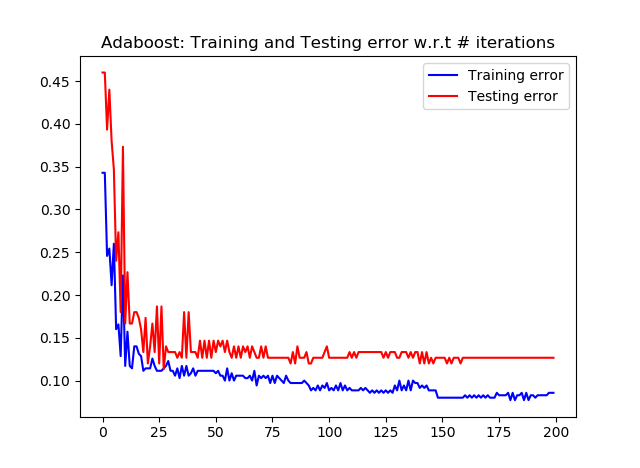
\includegraphics [width=0.38\linewidth]{train_test_error.png}
    \hfill
    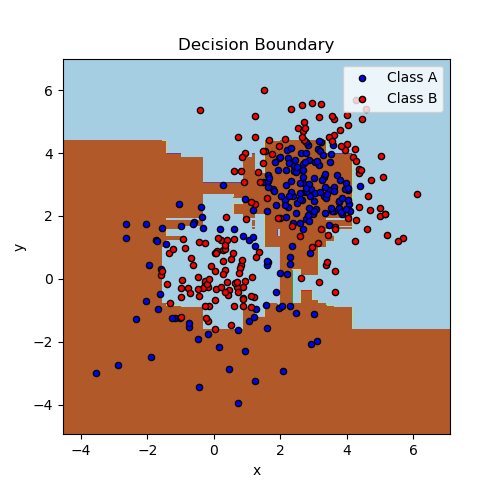
\includegraphics[width=0.3\linewidth]{decision_boundary2.png}
    \hfill
    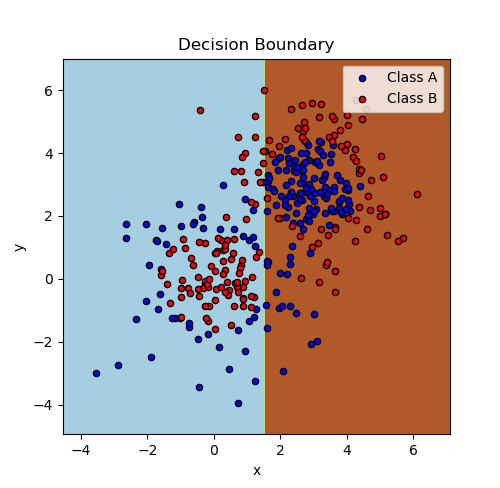
\includegraphics[width=0.3\linewidth]{decision_boundary.png}
    \caption{Visualization of adaboost results: (left) Training and Test errors per iteration; (middle) Decision boundary for the decision stump; (right) Adaboost decision boundary}
    \label{fig:adaboost}
\end{figure}



\end{enumerate}

\subsection*{Discussion}
I discussed with Radhika, Rizwan, and Qi Li while working on the homework problems.


\end{document}
